
In this section we derive our version of the standard quadrotor dynamic model given in \cite{hoffmann2004stanford} and \cite{pounds2002design} specific to the assumptions of level flight and $x^W \times y^W$ planar wind. 

\begin{figure}[t]
    \label{fig:QuadDiagram}
	\centering
	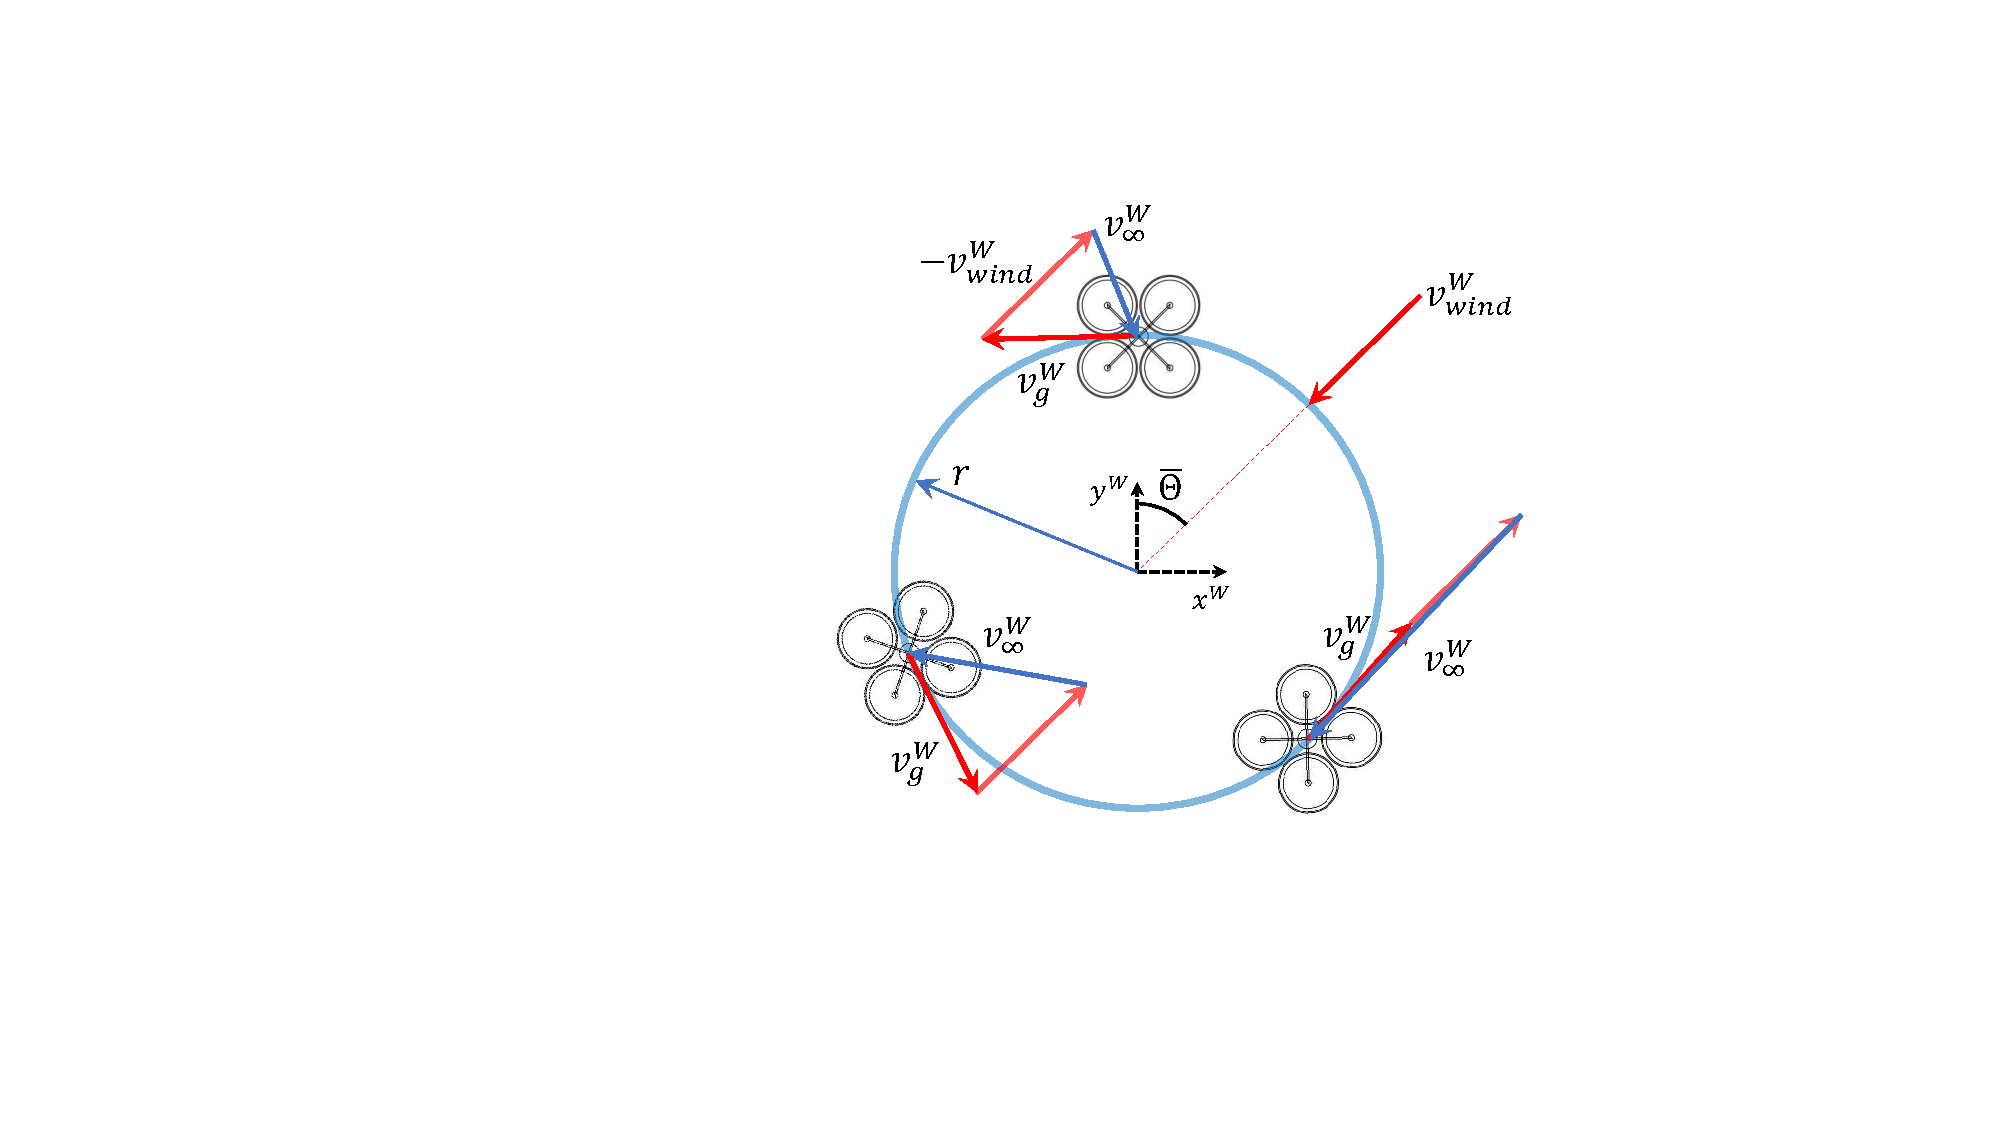
\includegraphics[width=0.5\textwidth, trim={14cm 5cm 8cm 2.5cm},clip]{coordinateDiagram.pdf}
	\caption{Definition of the coordinates used in our analysis. Frame $W$ is defined as a NEU world frame. Frame $B$ (not shown) is attached to the quadrotor's center of mass. Keeping with convention, $z^B$ points down and $x^B$ points forward so that positive pitch angles, $\theta$, correspond to pitching up. We define $\alpha$ as the angle between $\mathbf{v}_\infty^W$ and the rotor plane and $\mathbf{f}_D^W$ so that its direction is always equivalent to $v_\infty^W$. We define the radial position in the orbit by finding the mean wind heading for each experiment, $\bar{\Theta}$, and taking that as 0 radians. We can also see that $\mathbf{v}_\infty^W$ and $\alpha$ vary as the quadrotor moves around the orbit.}
\end{figure}

\subsection{Quadrotor dynamics}
We define two frames of reference, the NEU world frame, $W$, and the body fixed frame, $B$, attached to the quadrotor's center of mass. We also define $R$, a rotation matrix that describes the orientation of $B$ in $W$; $q^{w}=\left(x^W \text{, } y^W \text{, } z^W\right)$, a vector that gives the Cartesian position of $B$ in $W$; and $\mathbf{\omega}^B$, a vector that describes the angular velocity of $B$ with respect to $W$ in the body frame. We parameterize $R$ by the XYZ Euler angle sequence $\Theta=\left(\phi \text{, } \theta \text{, } \psi\right)$ corresponding to roll, pitch, and yaw respectively.

Assuming all four rotors are identical and neglecting blade flapping, each rotor will produce a thrust, $f_j^B \propto \sigma_j$, where $\sigma_j$ is the spin rate of the rotor. Additionally, each rotor will produce a torque, $\tau_j^B$, around each axis of $B$. Torques about $x^B$ and $y^B$ are moments proportional to $\sigma_j$, whereas torques about $z^B$ are pure torques proportional to the difference in spin rate between a rotor and its counter-rotor (i.e. $\sigma_2 - \sigma_4$ and $\sigma_1 - \sigma_3$).

We can then describe the translational and rotational dynamics of the quadrotor as a set of Newton-Euler equations
\begin{align}
    \label{NewtonEqn}
    m \ddot{\mathbf{q}}^W &= R \sum{\mathbf{f}_j^B} + \mathbf{f}_D^W - m\mathbf{g}^W \\
    \label{EulerEqn}
    I^B \dot{\mathbf{\omega}}^B &= -\mathbf{\omega} \times I^B \mathbf{\omega}^B + \sum{\mathbf{\tau}_j}^B
\end{align}
Where $I^B$ is the rotational inertia matrix, which is diagonal when the quadrotor is axisymmetric, the gravity vector is $\mathbf{g}^W=\left(0 \text{, } 0 \text{, } 9.8066\right) \text{ ms}^{-2}$, and $m$ is the mass of the quadrotor in kilograms.

\subsection{Assumption of level flight and planar wind}
By assuming level flight and that $v_{wind}$ is always on the $x^W \times y^W$ plane, we can make two simplifications to reduce our power model's number of parameters. First, rather than having to determine the angle of attack, $\alpha$, we can approximate its cosine and sine with \eqref{cosaoa} and \eqref{sinaoa}.
\begin{align}
	\label{cosaoa}
	\cos \alpha &= \cos \phi \cos \theta \\
	\label{sinaoa}
	\sin \alpha &= \sin \phi \sin \theta
\end{align}
Second, using \eqref{cosaoa} we can approximate the total thrust output by all four rotors, $T$, with just the roll and pitch angles.
\begin{align}
\label{totT}
T &= \frac{mg}{\cos \phi \cos \theta}
\end{align}
This means that our model requires no information about rotor spin rates to predict power consumption.

\subsection{Drag model}
Differing from \cite{tagliabue2019model} and \cite{schulz2015high}, we approximate our drag force with a function cubic in $v_\infty$ rather than quadratic. We did this to avoid overestimating the drag force at lower $v_\infty$ as shown in Fig. 3. We find that a cubic drag model reduces the error in $\hat{P}$ by 28\% on average across all our experiments.
\begin{align}
    \label{DragEqn}
    \mathbf{f}_D^W = \left(\mu_1 v_\infty + \mu_2 v_\infty^2 + \mu_3 v_\infty^3 \right)\frac{\mathbf{v}_\infty}{v_\infty} 
\end{align}
Where $\mu_1$, $\mu_2$, and $\mu_3$ are experimentally determined drag coefficients selected to make \eqref{DragEqn} approximate a more complex drag model such as the ones presented in \cite{huang2009aerodynamics}, \cite{bangura2012nonlinear}, or \cite{leishman2014quadrotors}. We assume that $\mathbf{f}_D^W$ is always co-linear with $\mathbf{v}_\infty^W$ and acts at the quadrotor's center of mass, producing no moments.

\begin{figure}[htbp]
	\centering
	\label{fig:DragModelRegression}
	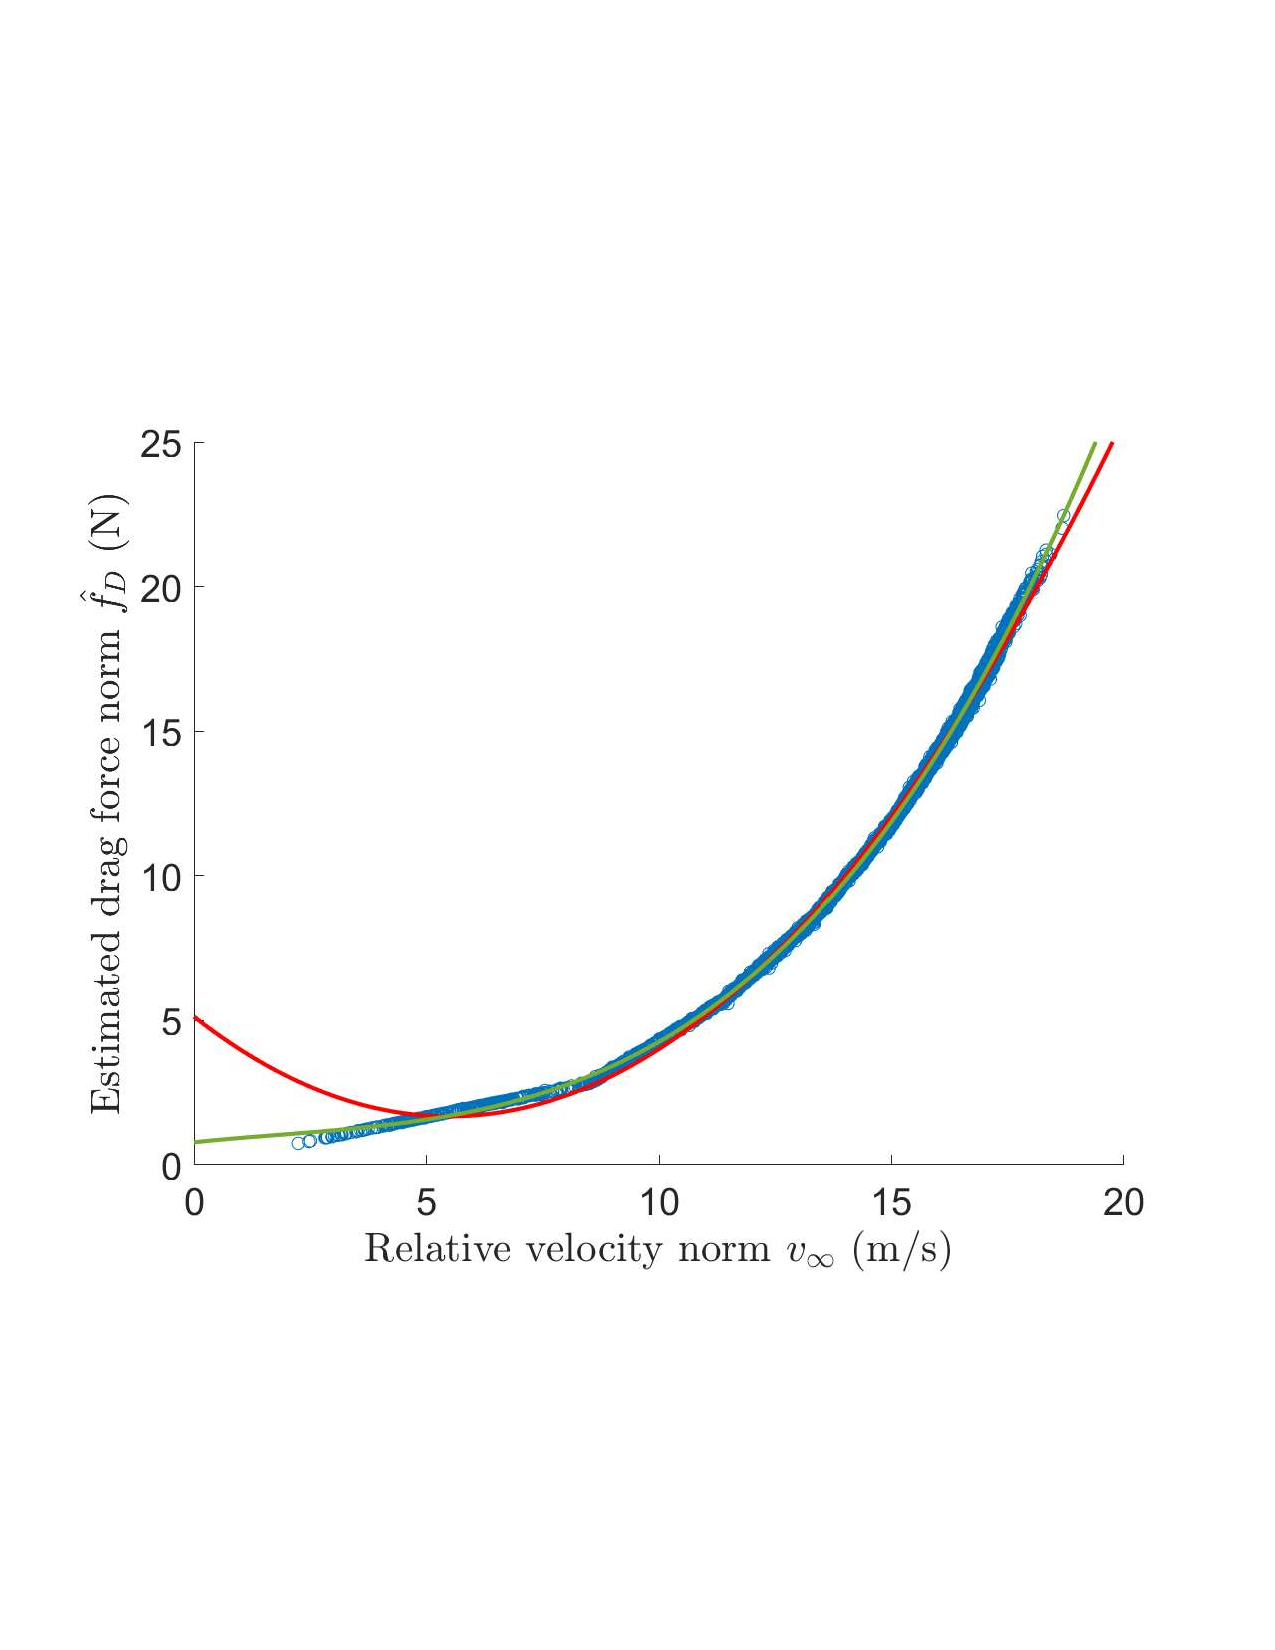
\includegraphics[width=0.5\textwidth, trim={1.25cm 6cm 1.5cm 6cm},clip]{dragModelRegressionWithQuad.pdf}
	\caption{Here we see that the quadratic fit (red) overestimates drag at lower $v_\infty$, whereas the cubic fit (green) closely matches the regression data for the whole range of $v_\infty$. The regression data was collected on level flights not in our experimental set; corresponding drag estimates are based on the residual dynamics of the quadrotor, where we assume thrust and acceleration are known. Drag coefficients for our vehicle: $\mu_1 = 0.1816 \textrm{, } \mu_2 = -0.02326 \textrm{, and } \mu_3 = 0.004045$.}
\end{figure}

\begin{figure*}[h]
	\centering
	\label{fig:relErrMeanGrad}
	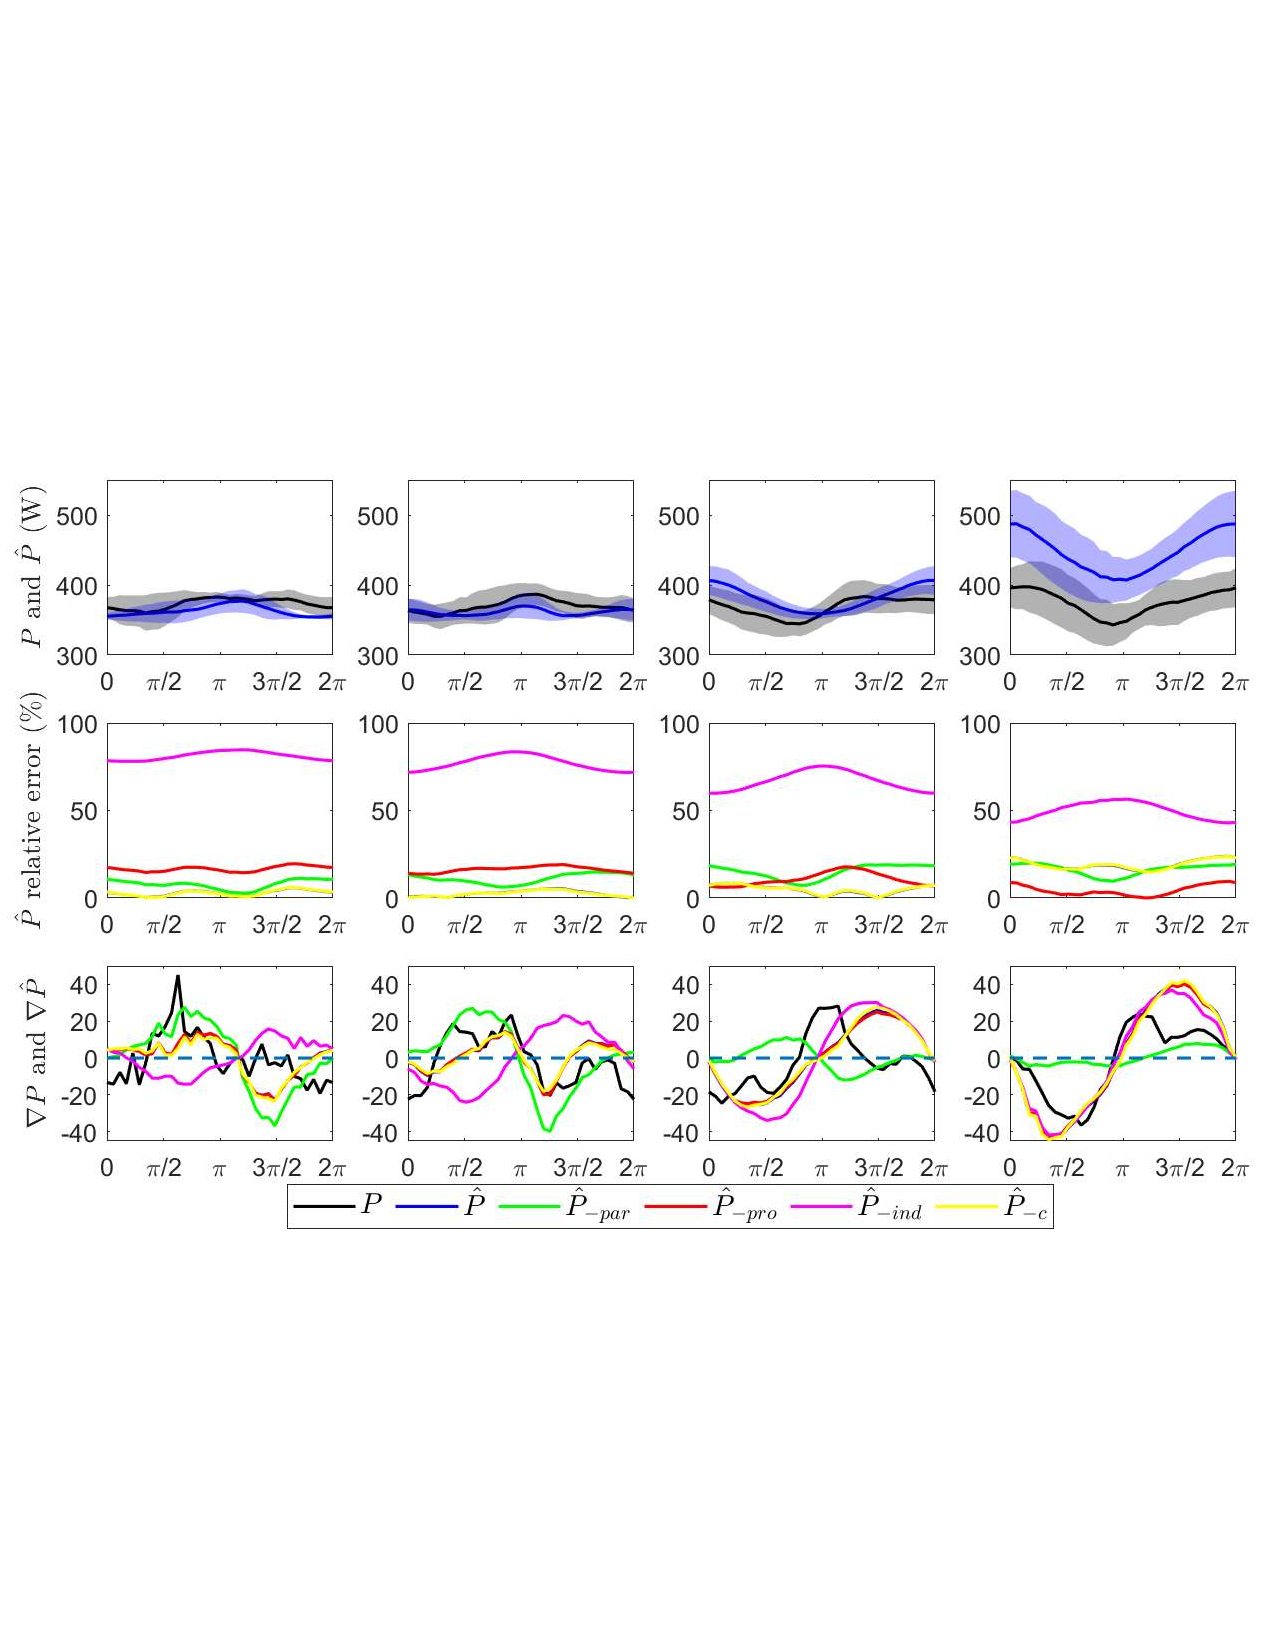
\includegraphics[width=\textwidth, trim={0cm 7cm 0cm 7cm}, clip]{meanCompareAll.pdf}
	\caption{Results for all non-hover flights separated by target $v_g$. Each plot is averaged over all altitudes and orbit radii flown. The x-axis is the quadrotor's position in the orbit in radians, descibed in Fig. 2. From left to right $v_g$ is 2 m/s, 4 m/s, 6 m/s, and 8 m/s. The subscript of $\hat{P}$ denotes which term is removed from the model. \textbf{Top}: Mean $P$ and $\hat{P}$ $\pm 1$ standard deviation. As $v_g$ increases so does the variance of $\hat{P}$. When $v_g$ is 8 m/s we also see a large increase in error, but as seen in the plot directly below, this error can be reduced by neglecting $P_{pro}$. \textbf{Middle}: Relative error between model estimates and measured $P$. We see there is little difference between the full model and the model with $P_c$ removed. Because all our flights were targeting a fixed altitude this is expected. It is also easy to see that the removal of $P_{ind}$ causes the largest error magnitude over all $v_g$. At 8 m/s we see that the inclusion of $P_{pro}$ degrades the accuracy of $\hat{P}$. \textbf{Bottom}: Gradient of $P$ and $\hat{P}$ with respect to position in the orbit. At lower $v_g$ we see that the exclusion of $P_{ind}$ causes the descent direction of the gradient to not lead towards minima in $P$. Although, as $v_g$ increases this problem dissipates. There is a larger amount of error when $P_{par}$ is removed, but in methods using gradient descent magnitude of the gradient is less important than the descent direction being correct.}
\end{figure*}

\subsection{Wind estimation}
The question of how to estimate a wind field onboard a quadrotor has been studied in great detail over the last decade, and continues to be a pressing question in aerial robotics \cite{waslander2009wind, huang2009aerodynamics, gonzalez2019sensing, xiang2016wind}. As seen in Section \ref{sec:Power}, our model is dependent on the output of these models to calculate the freestream velocity's norm, $v_\infty$. For these experiments, we use the output from DJI's built-in method for estimating wind velocity and heading. The accuracy of our model is directly dependent on the accuracy of DJI's model across varied flight regimes. 
